\documentclass[convert = false, tikz]{standalone}
\usepackage[utf8]{inputenc}
\usepackage{tikz}
\usetikzlibrary{automata, positioning, arrows}
 
\usepackage{../../../../style_automata}

% arara: pdflatex
% arara: latexmk: { clean: partial }
\begin{document}
    \tikzset{
    node distance=2.5cm, % specifies the minimum distance between two nodes.
    }
    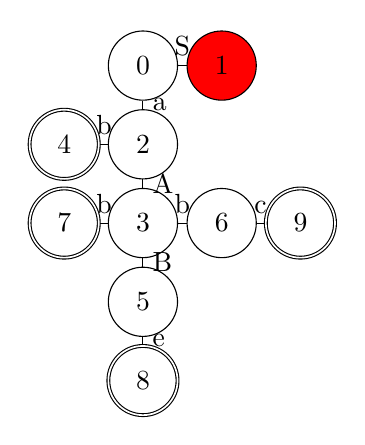
\begin{tikzpicture}
        \node[state] (0) {0};
        \node[state, fill=red, right of=0] (1) {1};
        \node[state, below of=0] (2) {2};
        \node[state, below of=2] (3) {3};
        \node[state, accepting, left of=2] (4) {4};
        \node[state, below of=3] (5) {5};
        \node[state, right of=3] (6) {6};
        \node[state, accepting, left of=3] (7) {7};
        \node[state, accepting, below of=5] (8) {8};
        \node[state, accepting, right of=6] (9) {9};
        \draw (0) edge[above] node{S} (1)
        (0) edge[right] node{a} (2)
        (2) edge[right] node{A} (3)
        (2) edge[above] node{b} (4)
        (3) edge[right] node{B} (5)
        (3) edge[above] node{b} (6)
        (3) edge[above] node{b} (7)
        (5) edge[right] node{e} (8)
        (6) edge[above] node{c} (9)
        ;

    \end{tikzpicture}
\end{document}

